
\documentclass[11pt]{article}


\usepackage{epsfig}
\usepackage{latexsym}
\usepackage{graphicx}
\DeclareGraphicsExtensions{.pdf,.png,.jpg}
\begin{document}

\title{Research Proposal}

\author{Nirbhay P. Tandon\\MSc. Data Science\\
    Research Title:\\Compare \& Contrast Existing Transformer\\ Architectures To Develop A New Architecture
}
\date{}
\maketitle


\begin{abstract}
Attention-based Transformer architectures have become the norm of current Natural Language Processing applications. Google began this trend back in 2017 with their paper \textit{Attention Is All You Need}\cite{atayl}, by introducing the Transformer architecture that works solely on attention mechanisms. The purpose of our work will be to explore a new kind of Transformer architecture. Compare \& contrast its performance against other architectures such as BERT\cite{bert}, RoBERTa\cite{roberta}, etc. that are also based on SQuAD 2.0 Dataset\cite{dataset}. Through our research, we aim to produce a new Transformer Architecture that has a better performance than existing models for Question Answering in a conversational manner.
\end{abstract}
\newpage
\tableofcontents
\newpage
\section{Introduction}\label{introduction}

The area of Natural language Processing has taken significant leaps in the last two decades. Work was done towards improving the ability of machine learning models to first recognize words, then sentences, followed by contextual understanding has led to several interesting \& novel approaches in the field. From early on neural networks to creating Long Short-Term Memory architectures\cite{originallstm} by Sepp Hochreiter \& Jurgen Schmidhuber helped in the mid-'90s that resolved the vanishing gradient problem of classical neural networks, we have come a long way.

The latest advancements in this field come from Google's research lab in the form of \textit{Transformers}\cite{atayl}. In their paper Attention Is All You Need\cite{atayl} Vasvani et. al demonstrated how replacing the \textit{encoder-decoder} based recurrent layers with \textit{multi-headed self-attention} based ones removes the need for recurrence and convolutions entirely.

We have divided our research proposal into 7 sections.
In Section \ref{introduction} we shall take a look at briefly introducing the concept \& why our work is necessary. Next, in Section \ref{backRR}, we outline the background work that has already been done in this field and how some of the papers relate to the work that has been done. We use this as an opportunity to highlight some of the shortcomings in current architectures \& modelling techniques. In Section \ref{aims} we briefly outline the aim of our proposed research. In Section \ref{researchMeth} we define in some detail the work that we will do to establish our research \& how we plan to quantify the work that shall be done. In Section \ref{expectedoutcomes} we have highlighted that our goal is to produce a new transformer architecture that performs better at Question Answering based tasks \& is capable of doing so in a conversational manner.
In Section \ref{resources} we have outlined the minimum hardware requirements along with the resources available to the author. Finally, in Section \ref{plan} we submit a Gantt Chart to outline our plan against the number of weeks.

\section{Background \& Related Research}\label{backRR}
In this section, we shall highlight why this research is being conducted, what has led us this far \& some of the interesting challenges that it poses. In \ref{back}, we briefly look at the history of Natural Language Processing \& how some of the challenges were addressed. In \ref{rr}, we look at the most interesting \& latest research that has gone into creating the Transformer architecture, identify some of the common patterns \& use that information to strategise our model in other sections.
\subsection{Background}\label{back}

\subsection{Related Research}\label{rr}

\begin{enumerate}
    \item A series of experiments have shown that these iterative methods provide enhanced performance in the word boundary detector which results in a significant improvement in speech recognition accuracy.\cite{chung}
    \item Long short-term memory\cite{lstm} and gated recurrent\cite{recurrent} neural networks in particular, have been firmly established as state of the art approaches in sequence modelling and transduction problems such as language modelling and machine translation.
    Aligning the positions to steps in computation time, they generate a sequence of hidden states $ ht $, as a function of the previous hidden state $ ht - l $ and the input for position $ t $. This inherently sequential nature precludes parallelization within training examples, which becomes critical at longer sequence lengths, as memory constraints limit batching across examples.
    The goal of reducing sequential computation forms the foundation of the Extended Neural GPU, ByteNet and ConvS2S, all of which use convolutional neural networks as basic building block, computing hidden representations in parallel for all input and output positions.
    Self-attention has been used successfully in a variety of tasks including reading comprehension, abstractive summarization, textual entailment and learning task-independent sentence representations. On the WMT 2014 English-to-German translation task, the big transformer model (Transformer in Table 2) outperforms the best previously reported models by more than 2.0 BLEU, establishing a new state-of-the-art BLEU score of 28.4.
    On the WMT 2014 English-to-French translation task, the big model achieves a BLEU score of 41.0, outperforming all of the previously published single models, at less than 1/4 the training cost of the previous state-of-the-art model.
    The authors set the maximum output length during inference to input length + 50, but terminate early when possible\cite{schuster}.The Transformer can be trained significantly faster than architectures based on recurrent or convolutional layers.
    On both WMT 2014 English-to-German and WMT 2014 English-to-French translation tasks, the authors achieve a new state of the art.
    In the former task the best model outperforms even all previously reported ensembles.
    Making generation less sequential is another research goals of ours\cite{atayl}
    \item Self-training methods such as ELMo (Peters et al, 2018), GPT (Radford et al, 2018), BERT (Devlin et al, 2019), XLM (Lample and Conneau, 2019), and XLNet (Yang et al, 2019) have brought significant performance gains, but it can be challenging to determine which aspects of the methods contribute the most.
    The authors present a replication study of BERT pretraining (Devlin et al, 2019), which includes a careful evaluation of the effects of hyperparmeter tuning and training set size.
    The two segments are presented as a single input sequence to BERT with special tokens delimiting them: [CLS ], x1, .
    BERT uses the ubiquitous transformer architecture (Vaswani et al, 2017), which the authors will not review in detail.
    Ashish Vaswani, Noam Shazeer, Niki Parmar, Jakob Uszkoreit, Llion Jones, Aidan N Gomez, Łukasz Kaiser, and Illia Polosukhin. 2017. Attention is all you need. In Advances in neural information processing systems.
    The authors use a transformer architecture with L layers.
    Each block uses A self-attention heads and hidden dimension H\cite{roberta}
    \item Increasing model size when pretraining natural language representations often results in improved performance on downstream tasks. At some point further model increases become harder due to GPU. Proposed methods lead to models that scale much better compared to the original BERT, a self-supervised loss that focuses on modeling inter-sentence coherence. A Lite BERT (ALBERT) architecture that has significantly fewer parameters than a traditional BERT architecture. These results show that weight-sharing has an effect on stabilizing network parameters. Inter-sentence modeling is an important aspect of language understanding, but we propose a loss based primarily on coherence. We have convincing evidence that sentence order prediction is a more consistently-useful learning task that leads to better language representations, we hypothesize that there could be more dimensions not yet captured by the current self-supervised training losses that could create additional representation power for the resulting representations. 4.2.2 DOWNSTREAM EVALUATION Following Yang et al (2019) and Liu et al (2019), we evaluate our models on three popular benchmarks: The General Language Understanding Evaluation (GLUE) benchmark (Wang et al, 2018), two versions of the Stanford Question Answering Dataset (SQuAD; Rajpurkar et al, 2016; 2018), and the ReAding Comprehension from Examinations (RACE) dataset (Lai et al, 2017). \cite{albert}
    \item Machine reading comprehension has become a central task in natural language understanding, fueled by the creation of many large-scale datasets. Question 2: “What was the name of the 1937 treaty?” Plausible Answer: Bald Eagle Protection Act even produced systems that surpass human-level exact match accuracy on the Stanford Question Answering Dataset (SQuAD), one of the most widely-used reading comprehension benchmarks. These systems are still far from true language understanding. Models only need to select the span that seems most related to the question, instead of checking that the answer is entailed by the text. The authors evaluated three existing model architectures: the BiDAF-No-Answer (BNA) model proposed by Levy et al (2017), and two versions of the DocumentQA No-Answer (DocQA) model from Clark and Gardner (2017), namely versions with and without ELMo (Peters et al, 2018)
    These models all learn to predict the probability that a question is unanswerable, in addition to a distribution over answer choices.
    The authors find this strategy does slightly better than taking the argmax prediction, possibly due to the different proportions of negative examples at training and test time. A state-of-the-art model achieves only 66.3\% F1 score when trained and tested on SQuAD 2.0, whereas human accuracy is 89.5\% F1, a full 23.2 points higher.
    When evaluating on the test set, the authors use the threshold that maximizes F1 score on the development set.
    Following Rajpurkar et al (2016), the authors report average exact match and F1 scores.  SQuAD 2.0 forces models to understand whether a paragraph entails that a certain span is the answer to a question.
    Relation extraction systems must understand when a possible relationship between two entities is not entailed by the text (Zhang et al, 2017).
    Jia and Liang (2017) created adversarial test examples that fool models trained on SQuAD 1.1. Models that are trained on similar examples are not fooled by their method.
    The adversarial examples in SQuAD 2.0 are difficult even for models trained on examples from the same distribution. \cite{dataset}
    \item Language model pre-training has been shown to be effective for improving many natural language processing tasks (Dai and Le, 2015; Peters et al, 2018a; Radford et al, 2018; Howard and Ruder, 2018).
    The two approaches share the same objective function during pre-training, where they use unidirectional language models to learn general language representations. The authors present BERT fine-tuning results on 11 NLP tasks. 4.1 GLUE. The General Language Understanding Evaluation (GLUE) benchmark (Wang et al, 2018a) is a collection of diverse natural language understanding tasks.
    The authors present BERT fine-tuning results on 11 NLP tasks.
    The General Language Understanding Evaluation (GLUE) benchmark (Wang et al, 2018a) is a collection of diverse natural language understanding tasks.
    To fine-tune on GLUE, the authors represent the input sequence as described, and use the final hidden vector C equals RH corresponding to the first input token ([CLS]) as the aggregate representation.
    The only new parameters introduced during fine-tuning are classification layer weights W equals RK x H , where K is the number of labels. The best performing method concatenates the token representations from the top four hidden layers of the pre-trained Transformer, which is only 0.3 F1 behind fine-tuning the entire model.
    This demonstrates that BERT is effective for both finetuning and feature-based approaches.
    Using only the RND strategy performs much worse than the strategy as well. Recent empirical improvements due to transfer learning with language models have demonstrated that rich, unsupervised pre-training is an integral part of many language understanding systems.
    These results enable even low-resource tasks to benefit from deep unidirectional architectures.
    The authors' major contribution is further generalizing these findings to deep bidirectional architectures, allowing the same pre-trained model to successfully tackle a broad set of NLP tasks.\cite{bert}
    \item Recurrent networks can in principle use their feedback connections to store representations of recent input events in form of activations (short-term memory", as opposed to long-term memory" embodied by slowly changing weights).
    This is potentially significant for many applications, including speech processing, non-Markovian control, and music composition (e.g., Mozer 1992).
    With conventional Back-Propagation Through Time" (BPTT, e.g., Williams and Zipser 1992, Werbos 1988) or Real-Time Recurrent Learning". The authors use 3 different, randomly generated pairs of training and test sets. With each such pair the authors run 10 trials with different initial weights. The difficult task is of a type that has never been solved by other recurrent net algorithms. It shows that LSTM can solve long time lag problems involving distributed, continuous valued representations.
    Long Short-Term Memory
    Once block 1 is called and closed, this fact will become visible to block 2. The efficient truncated backprop version of the LSTM algorithm will not solve problems similar to strongly delayed XOR problems", where the goal is to compute the XOR of two widely separated inputs that previously occurred somewhere in a noisy sequence.
    By generating an appropriate negative connection between memory cell output and input, LSTM can give more weight to recent inputs and learn decays where necessary.Each memory cell's internal architecture guarantees constant error ow within its constant error carrousel CEC, provided that truncated backprop cuts o error ow trying to leak out of memory cells
    This represents the basis for bridging very long time lags.
    It will be interesting to augment sequence chunkers. \cite{schmid}
    \item  Relation extraction systems populate knowledge bases with facts from an unstructured text corpus.
    When the type of facts are predefined, one can use crowdsourcing (Liu et al, 2016) or distant supervision (Hoffmann et al, 2011) to collect examples and train an extraction model for each relation type.
    The relation educated at(x, y) can be mapped to “Where did x study?” and “Which university did x graduate from?”. The authors' goal is to find a set of text spans A in s for which R(e, a) holds for each a equals A. To understand how well the method can generalize to unseen data, the authors design experiments for unseen entities, unseen question templates, and unseen relations. The authors test the method’s ability to generalize to new descriptions of the same relation, by holding out a question template for each relation during training. Some recent QA datasets were collected by expressing knowledge-base assertions in natural language.
    The Simple QA dataset (Bordes et al, 2015) was created by annotating questions about individual Freebase facts (e.g. educated at(T uring, P rinceton)), collecting roughly 100,000 natural-language questions to support QA against a knowledge graph.
    To the best of the knowledge, this is the first robust method for collecting a question-answering dataset by crowd-annotating at the schema level.The authors showed that relation extraction can be reduced to a reading comprehension problem, allowing them to generalize to unseen relations that are defined on-the-fly in natural language.
    To support future work in this avenue, the authors make the code and data publicly available.\cite{levy}
    \item Question answering is an important end-user task at the intersection of natural language processing (NLP) and information retrieval (IR). Results presented in Tables 2 and 3 clearly demonstrate the strength of the FastQA + char-emb. (FastQA) system. It is very competitive to previously established stateof-the-art results on the two datasets and even improves those for NewsQAWe introduced a simple, context/type matching heuristic for extractive question answering which serves as guideline for the development of two neural baseline system. FastQA, our recurrent neural network (RNN)-based system turns out to be an efficient neural baseline architecture for extractive question answering. It combines two simple ingredients necessary for building a currently competitive QA system: a) the awareness of question words while processing the context and b) a composition function that goes beyond simple bag-of-words modeling. We argue that this important finding puts results of previous, more complex architectures as well as the complexity of recent QA datasets into perspective\cite{wiese}
    \item As machine reading comprehension tasks with unanswerable questions stress the importance of answer verification in Machine reading comprehension modeling, this paper devotes itself to better verifieroriented MRC task-specific design and implementation for the first time.\cite{zhang2} Machine reading comprehension (MRC) aims to teach machines to answer questions after comprehending given passages (Hermann et al 2015; Joshi et al 2017; Rajpurkar, Jia, and Liang 2018), which is a fundamental and longstanding goal of natural language understanding (NLU). In terms of powerful enough PrLMs like ALBERT and ELECTRA, the Retro-Reader significantly outperforms the baselines with p-value < 0.01,8 and achieves new state-of-the-art on the SQuAD2.0 challenge..
    The authors' method shows consistent improvements over the baselines and achieves new state-of-the-art results
    Retro-Reader on ALBERT and Retro-Reader on ELECTRA denote the final models, which are respectively the ALBERT and ELECTRA based retrospective reader composed of both sketchy and intensive reading modules without question-aware matching for simplicity.
    The authors make the following observations: 1) The authors' implemented ALBERT and ELECTRA baselines show the similar EM and F1 scores with the original num- All HasAns NoAns. EM F1 EM F1 EM F1 BERT + E-FV + RV ALBERT\cite{zhang}
    \item Pre-trained word representations (Mikolov et al, 2013; Pennington et al, 2014) are a key component in many neural language understanding models.
    Learning high quality representations can be challenging
    They should ideally model both (1) complex characteristics of word use, and (2) how these uses vary across linguistic contexts.
    The authors use vectors derived from a bidirectional LSTM that is trained with a coupled language model (LM) objective on a large text corpus.
    For this reason, the authors call them ELMo (Embeddings from Language Models) representations.
    The authors learn a linear combination of the vectors stacked above each input word for each end task, which markedly improves performance over just using the top LSTM layer. Adding ELMo establishes a new state-of-the-art result, with relative error reductions ranging from 6 - 20\% over strong base models.
    This is a very general result across a diverse set model architectures and language understanding tasks.
    The authors' baseline model (Clark and Gardner, 2017) is an improved version of the Bidirectional Attention Flow model in Seo et al (BiDAF; 2017).
    A 11 member ensemble pushes F1 to 87.4, the overall state-of-the-art at time of submission to the leaderboard. The increase of 4.7\% with ELMo is significantly larger the 1.8\% improvement from adding CoVe to a baseline model (McCann et al, 2017).  The authors have introduced a general approach for learning high-quality deep context-dependent representations from biLMs, and shown large improvements when applying ELMo to a broad range of NLP tasks.
    Through ablations and other controlled experiments, the authors have confirmed that the biLM layers efficiently encode different types of syntactic and semantic information about wordsin-context, and that using all layers improves overall task performance
    \cite{contextualized}
\end{enumerate}

\newpage
\newpage
\section{Aims \& Objectives}\label{aims}

The main aim of this research is to propose a new transformer architecture that can perform better at conversational Question \& Answering from the SQuAD 2.0 dataset\cite{dataset}.
We shall:
\begin{enumerate}
    \item Implement the existing models that are available via libraries such as HuggingFace\cite{hfTransformers}, PyTorch \& Tensorflow, run the SQuAD 2.0\cite{dataset}
    \item Obtain F1, validation, etc. scores for existing models \& treat them as our benchmark scores
    \item Identify drawbacks of the current architectures
    \item Design our architecture \& evaluate its performance
    \item Fine-tune the architecture, re-evaluate \& report improvements
    \item Compare the results of our Transformer model with the benchmark scores.
\end{enumerate}
We hope to establish our proposed transformer architecture as a competent enough contender to be used within both industry \& academia.
\section{Research Methodology}\label{researchMeth}

To implement this research we shall break the project down into 5 phases. These are outlined below.
\subsection{Literature Review}\label{litrev}

In this phase, we will
\begin{enumerate}
    \item Review the research that has been published already around the different kinds of architectures
    \item Shortlist some of the most widely used ones, compare their results using the SQuAD 2.0 \cite{dataset} \& outline the pros and cons of each of these architectures.
\end{enumerate}
The rationale is to review \& understand as much of the previously established research as possible so that we can avoid potential pitfalls, not duplicate our efforts by reinventing the wheel \& organize a better approach to perform our research. A lot of the background work available has already been highlighted in
\subsection{Research Benchmarks}\label{benchmarks}
Here we shall focus on obtaining benchmark scores for the shortlisted architectures above using the dataset\cite{dataset}. The parameters used will be validation \& test set scores of the models. The training shall be carried out on each of the models for 100 epochs. We shall also look at the specificity/recall of these results to better understand if our work was done correctly or not.
\subsection{Architecture Creation}\label{architecturecreation}
In this section we will:

\begin{enumerate}
    \item{Mathematically model a new transformer architecture}
    \item{Code the architecture}
    \item{Run sample dataset to identify base benchmarks}
    \item{Run the SQuAD 2.0 dataset\cite{dataset} to obtain 1st pass performance benchmarks}
    \item{Document architecture performance, identify pros \& cons}
\end{enumerate}
\subsection{Architecture Refinement}\label{refinement}
In this phase, we will focus on:
\begin{enumerate}
    \item{Reviewing the results from the previous section}
    \item{Identifying the areas of improvement}
    \item{Hypothesise the improvements \& implement them in the architecture}
    \item{Run the SQuAD 2.0 dataset\cite{dataset} to obtain new performance benchmarks}
    \item{Document architecture performance, identify pros \& cons}
\end{enumerate}
\subsection{Research Findings}\label{findings}
In this subsection, we shall highlight the achievements of our research \& draw comparisons to the benchmarks we obtained in \ref{benchmarks}.
\subsection{Conclusion}\label{conclusions}

Finally, here we aim to successfully conclude that our model performs better than existing models.
\section{Expected Outcomes}\label{expectedoutcomes}

We expect that our created model is at-par, if not better performing than existing models for Question Answering based problems.
\section{Requirements \& Resources}\label{resources}

To successfully deliver on our research we will be utilizing the following hardware:
\begin{itemize}
    \item EVGA GeForce RTX 2070 SUPER KO GAMING, 08G-P4-2072-KR, 8GB GDDR6, Dual Fans\cite{2070}. This graphics card is based on the Nvidia "Turing" architecture \& has 2560 CuDA cores.
    \item Intel 10700 processor. 8 cores, 16 threads, 16M cache\cite{intel}.
    \item VENGEANCE® LPX 8GB (1 x 8GB) DDR4 DRAM 2400MHz C14 Memory Kit - Black\cite{ram}. 8GB x 4, 32 GB total.
    \item Minimum 650W power supply.
    \item Minimum B550 Motherboard architecture. We will use the Asus Prime B550 motherboard\cite{asus}.
\end{itemize}

The above hardware is available to the author \& any changes to the same will be notified/highlighted in the subsequent reports.
\section{Research Plan}\label{plan}

Shown on the next page is the Gantt Chart highlighting the research stages \& timelines.\\
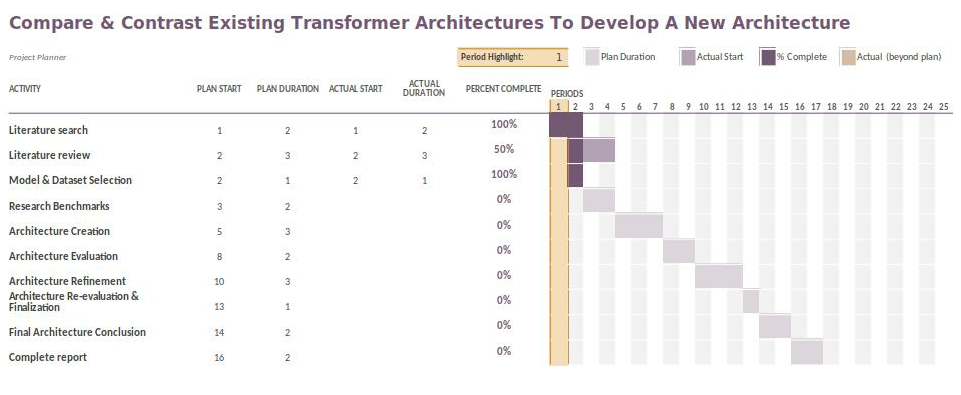
\includegraphics[width=180mm,height=120mm,angle=90]{g2}
\newpage
\bibliographystyle{plain}
\bibliography{Research_Proposal}

\end{document}
